
%%%%%%%%%%%%%%%%%%%%%%%%%%%%%%%%%%%%%%%%%
% University/School Laboratory Report
% LaTeX Template
% Version 3.1 (25/3/14)
%
% This template has been downloaded from:
% http://www.LaTeXTemplates.com
%
% Original author:
% Linux and Unix Users Group at Virginia Tech Wiki 
% (https://vtluug.org/wiki/Example_LaTeX_chem_lab_report)
%
% License:
% CC BY-NC-SA 3.0 (http://creativecommons.org/licenses/by-nc-sa/3.0/)
%
%%%%%%%%%%%%%%%%%%%%%%%%%%%%%%%%%%%%%%%%%

%----------------------------------------------------------------------------------------
%	PACKAGES AND DOCUMENT CONFIGURATIONS
%----------------------------------------------------------------------------------------

\documentclass{article}
\usepackage[margin=1.25in]{geometry}
\usepackage{hyperref}
\usepackage[version=3]{mhchem} % Package for chemical equation typesetting
\usepackage{siunitx} % Provides the \SI{}{} and \si{} command for typesetting SI units
\usepackage{graphicx} % Required for the inclusion of images
\usepackage{natbib} % Required to change bibliography style to APA
\usepackage{amsmath} % Required for some math elements 

\setlength\parindent{1em} % Removes all indentation from paragraphs
\setlength{\parskip}{1em}
\renewcommand{\labelenumi}{\alph{enumi}.} % Make numbering in the enumerate environment by letter rather than number (e.g. section 6)

%\usepackage{times} % Uncomment to use the Times New Roman font

%----------------------------------------------------------------------------------------
%	DOCUMENT INFORMATION
%----------------------------------------------------------------------------------------

\title{Check-in} % Title

\author{Weixiong Zheng} % Author name

\date{April 24, 2018} % Date for the report

\begin{document}

\maketitle % Insert the title, author and date
% If you wish to include an abstract, uncomment the lines below
% \begin{abstract}
% Abstract text
% \end{abstract}

%----------------------------------------------------------------------------------------
%	SECTION 0
%----------------------------------------------------------------------------------------
\section{Updates on previous goals}
There were a bunch of goals set up from last check-in.

\begin{itemize}
	\item new/more reasonable designs of classes/namespaces during restart
	\item adding pin-resolved mesh functionality.
	\item helping figure out Marissa's code bugs
\end{itemize}
%----------------------------------------------------------------------------------------
%	SECTION 1
%----------------------------------------------------------------------------------------
\section{Progress up to now}
\subsection{Introduction slides}
I've been trying to create an introduction slides. A draft without in-detail testing section has been created but still needs a lot of re-reading and revisions.

\subsection{Continuous progress on restarting}
The new design mainly involves better using namespaces to contain free functions (rather than using static member method) and more importantly, a global {\tt dealii::ParameterHandler} object. Current implementation for every class has an argument as {\tt dealii::ParameterHandler \&prm}. From Josh's idea, I implemented a global object in the {\tt bparams} namespace ({\tt dealii::ParameterHandler bparams::GlobPrm}). Modifying class constructors to use this global object is trivial, however, all the testings needs to be modified accordingly. So the plan is to get Alex coding with me on this part to finish it.

Just as planned and doing it continuously. Yet, there's a big trunk of 
testing code that needs to be modified accordingly with the design in restart

\subsection{Last experiment on pin-resolved mesh}
After merging rectangle pin meshing, the last experiment was performed to generate hexagonal pin. Added three trivial PRs to deal.II so in the future we can use them directly from deal.II instead of keeping BART unnecessarily bulky. 

Thereafter, another experiment was performed on making hexagonal pin, which is useful when simulating fast reactors. See the demo in Figure\ 1.

\begin{figure}
	\centering
%	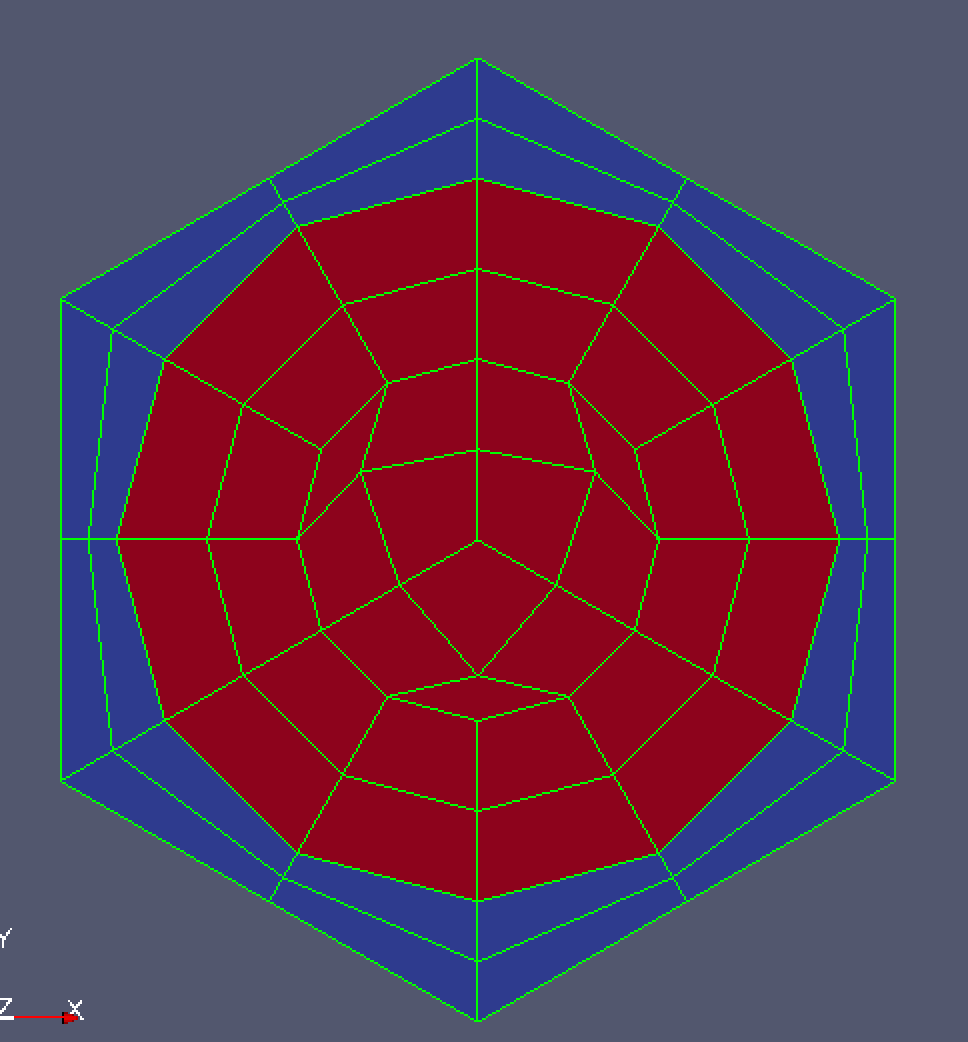
\includegraphics[width=0.5\textwidth]{hex-pin}
	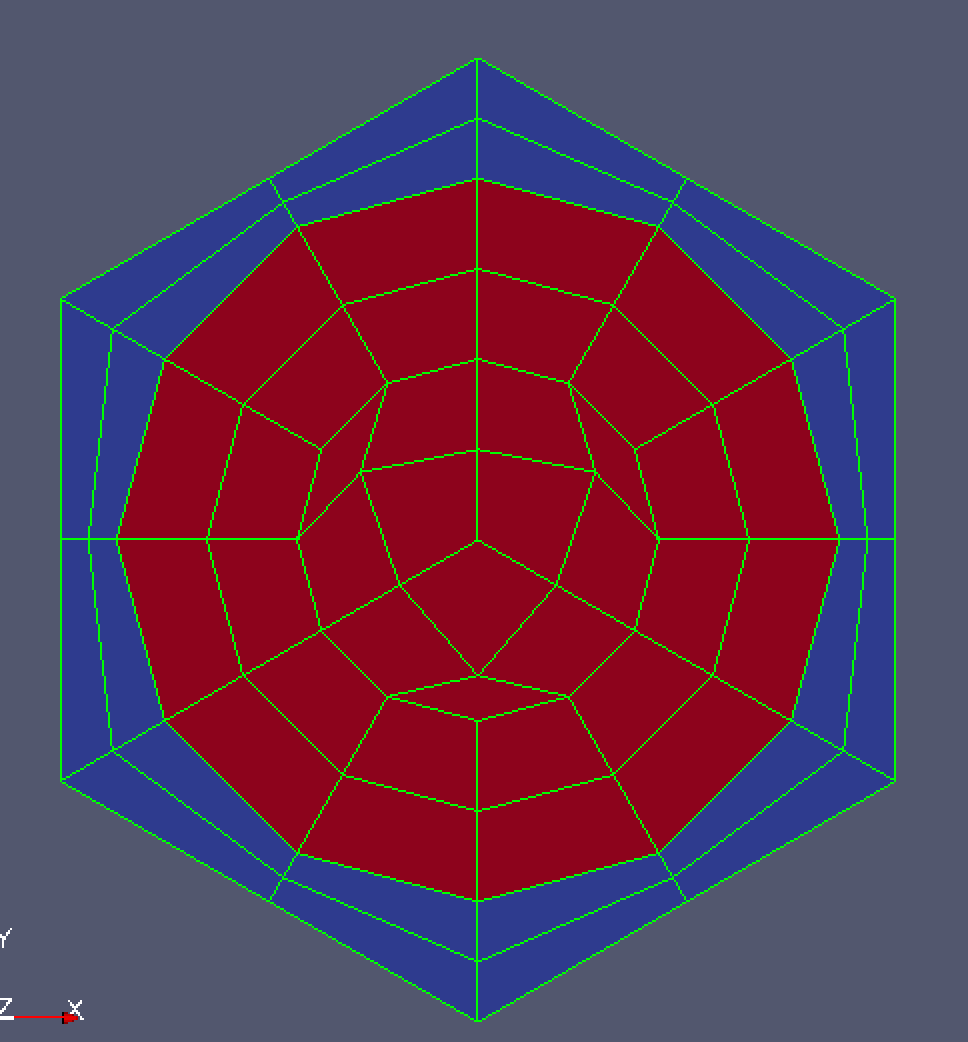
\includegraphics[scale=0.35]{hex-pin}
	\caption{Hexagonal pins}
\end{figure}

The hex-related things could be a interesting directions for future development and research on fast reactors.

\subsection{Students}
Marissa seems to get things work after our hours of struggle. We finally realized that she had fixed the bug at some point but we kept thinking the implementation was wrong. It turned out to be the plotting functionality flaws of Python functions (or how Marissa used it).

I got a talk with Alex and assigned a task moving {\tt MaterialProperties} class to {\tt restart} branch.
%----------------------------------------------------------------------------------------
%	SECTION 2
%----------------------------------------------------------------------------------------
\section{Things you need from Rachel}


%----------------------------------------------------------------------------------------
%	SECTION 3
%----------------------------------------------------------------------------------------
\section{Goals/Things will be going on}
I will just keep moving on as planned so we can finish restarting soon. Also, I may set up a para-coding with Alex if necessary to help him get things moving on.

%----------------------------------------------------------------------------------------
%	SECTION 4
%----------------------------------------------------------------------------------------
%\section{Links to any related materials}



%----------------------------------------------------------------------------------------
%	BIBLIOGRAPHY
%----------------------------------------------------------------------------------------

%\bibliographystyle{apalike}
%
%\bibliography{sample}

%----------------------------------------------------------------------------------------


\end{document}